\documentclass[sigconf,10pt]{acmart}
\settopmatter{printacmref=false}
\renewcommand\footnotetextcopyrightpermission[1]{}
\setcopyright{none}
\pagestyle{plain}

\usepackage{subfigure,cleveref}
\crefname{section}{\S}{\S\S}
\usepackage{amsmath,multirow}
\usepackage{booktabs}
\usepackage{graphicx}
\usepackage{xcolor}
\usepackage{xspace}
\usepackage{placeins}
\usepackage{tikz}
\usetikzlibrary{arrows.meta,calc,positioning}
\usepackage{algorithm}
\usepackage[noend]{algpseudocode}
\algrenewcommand{\algorithmiccomment}[1]{\hfill\texttt{//} #1}
\algrenewcommand{\algorithmicrequire}{\textbf{Input:}}
\algrenewcommand{\algorithmicensure}{\textbf{Output:}}

\newcommand{\system}{ViewTree\xspace}
\newcommand{\worldmem}{world memory\xspace}
\newcommand{\placeholderbox}[2]{%
	\fcolorbox{red}{white}{\parbox[c][#1][c]{0.91\columnwidth}{%
			\centering\color{red}\small #2}}}

\begin{document}
	
	%\title{ViewTree: Spatial Reasoning over an Explicit Scene Memory via Confidence-Guided Camera Walks}
	\title{ViewTree: On-Device Spatial Intelligence via Confidence-Guided Camera Walks over Explicit Scene Memory}	
		%	\title{ViewTree: Spatial Reasoning over an Explicit Scene Memory via Confidence-Guided Camera Walks}
	\begin{abstract}
		
	\end{abstract}
	
	\maketitle
	\pagestyle{plain}
	
	\section{Introduction}
	Many mobile and embedded devices nowadays use visual streams as the input to vision-language models (VLMs) to perceive the physical world and guide device actions \cite{}. Instead of using cloud AI services, executing VLMs locally protects data privacy and avoids possible network disruptions, both of which are important to interactive applications such as robotic manipulation \cite{zheng2025survey, yuan2024cross}, navigation \cite{simon2023mononav}, AR/VR assistants \cite{skurowski2024energy, liu2019edge} and mobile video analytics \cite{wang2025empowering}. 
	
	Being different from traditional appearance-based visual tasks such as object detection \cite{cheng2024yolo, liu2024grounding} and semantic segmentation \cite{kirillov2023segment,liu2024grounding} shown in Figure \ref{fig:all_scenarios}(a), these emerging applications build on the ability of \textbf{spatial intelligence}, which comprehends the 3D physical properties of the environment and geometric relations (e.g., distance, orientation, and relative positioning) between objects in different views. For example in Figure \ref{fig:all_scenarios}(b), to identify the correct box to retrieve, a robot translates the allocentric input command into egocentric actions, requiring correct understanding of the spatial relationships across the camera's view and robot's view. Similarly, a wearable AR assistant estimates the object's 3D dimensions to determine whether it fits into the elevator, and a search-and-rescue drone builds a 3D map of an unknown area to report the survivor's location relative to the landmarks. 
	
	\begin{figure}
		\centering
		% First subfigure
		\subfigure[Traditional visual tasks of object detection and recognition]{
			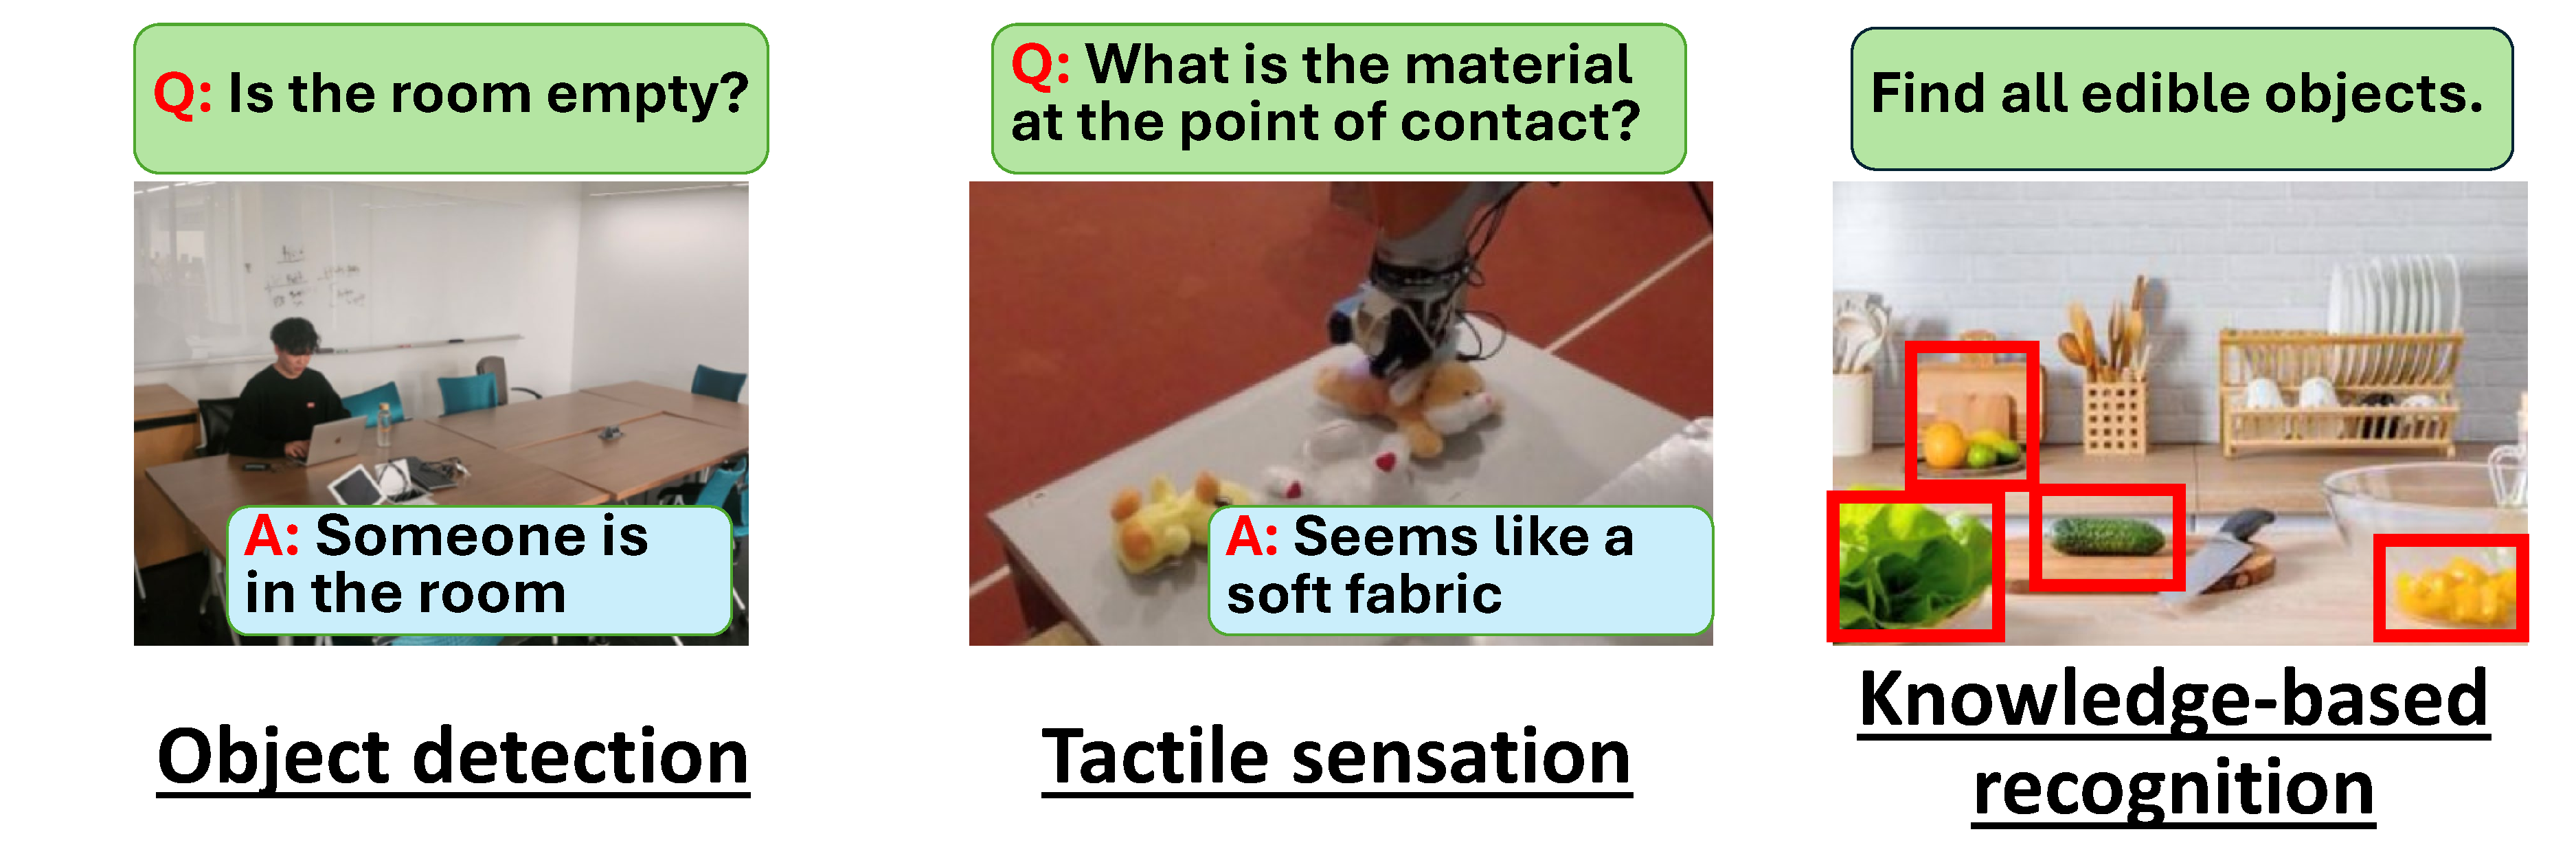
\includegraphics[width=0.85\linewidth]{figures/traditional_task.pdf}
			\label{fig:traditional_task}
		}
		\vspace{-0.2in}
		% Second subfigure
		\subfigure[Emerging visual tasks based on spatial intelligence]{
			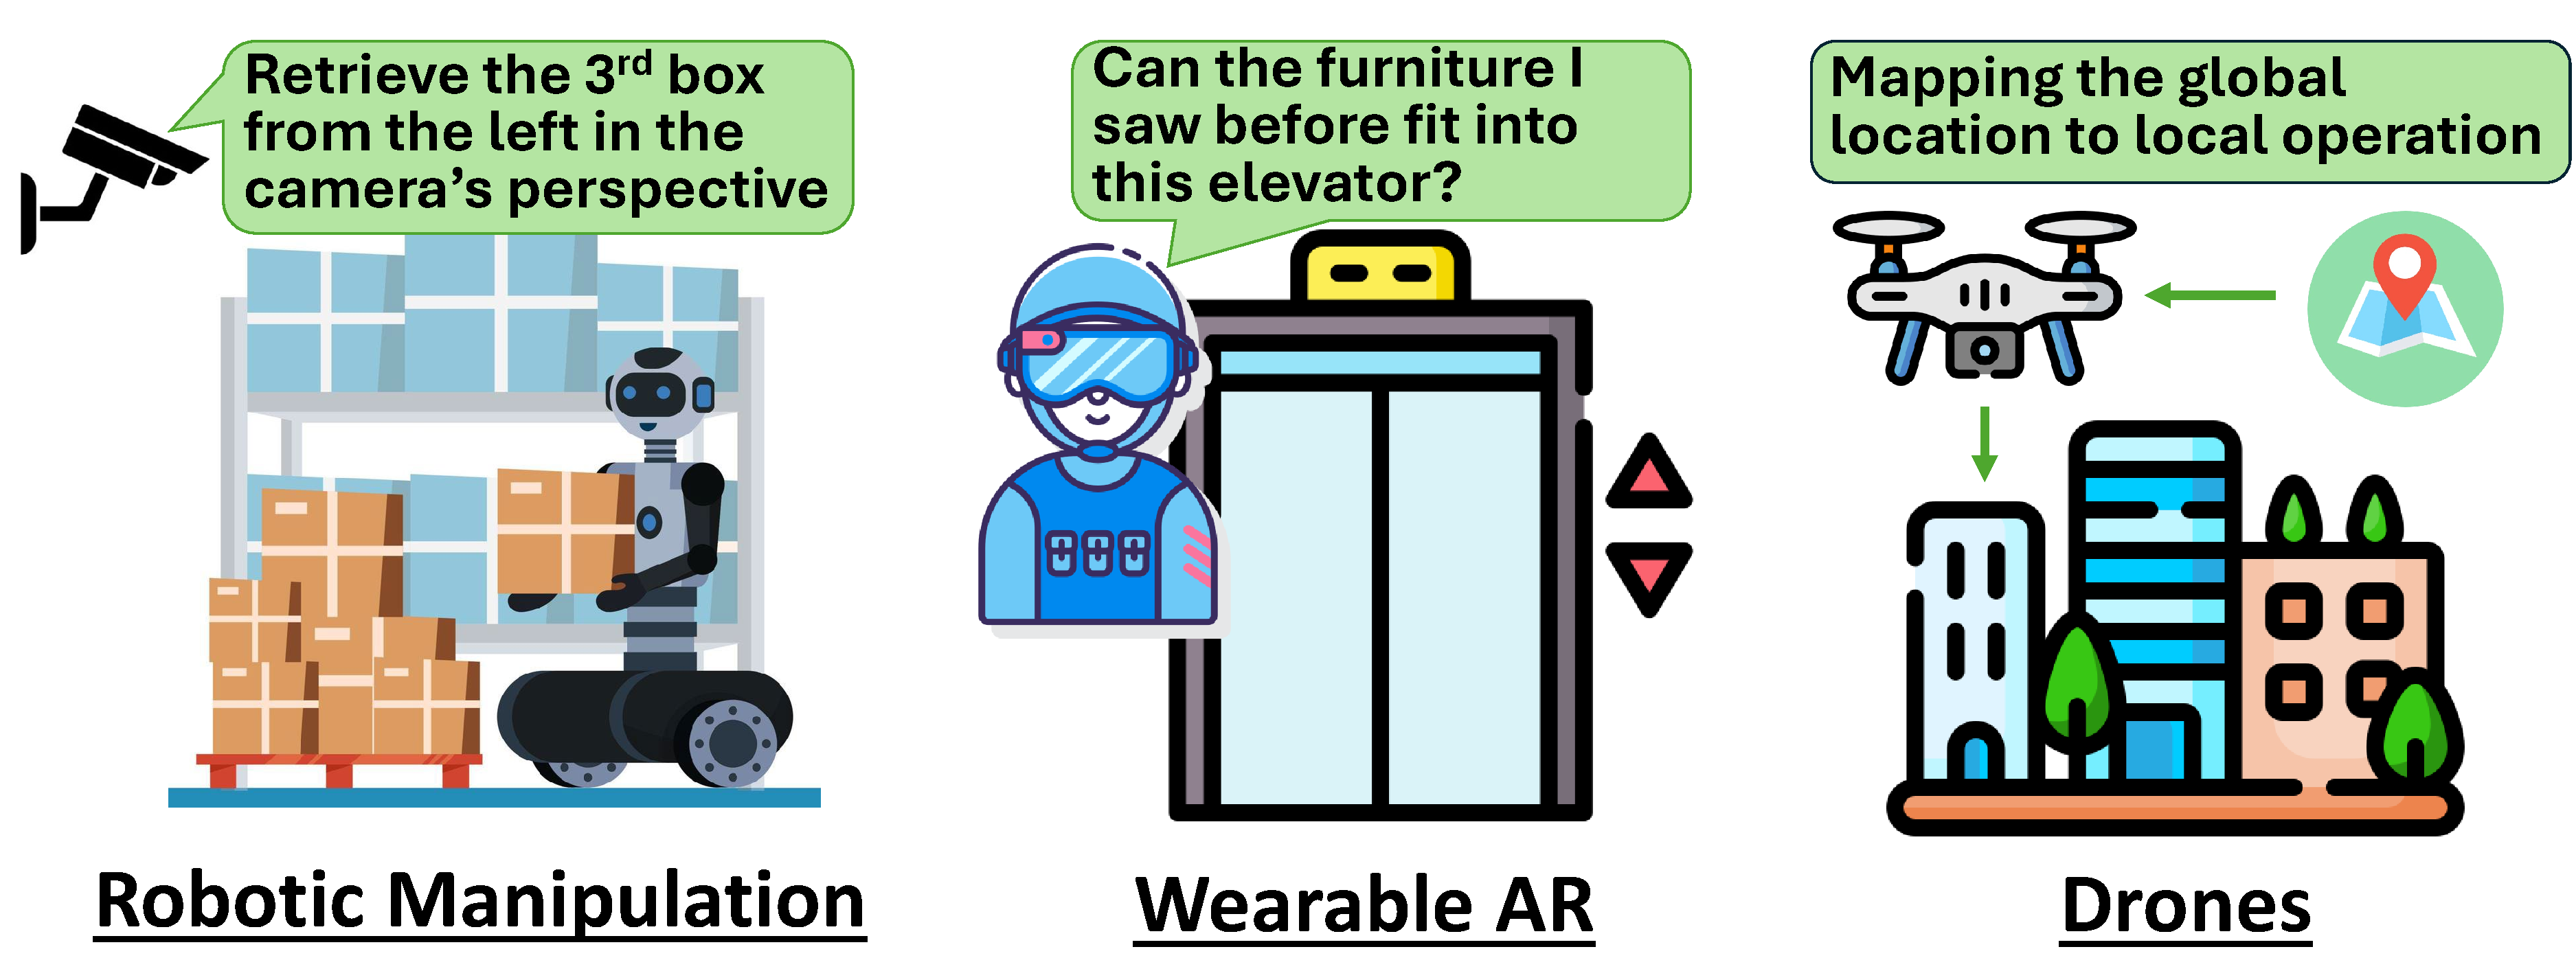
\includegraphics[width=0.85\linewidth]{figures/application.pdf}
			\label{fig:reasoning_task}
		}
		%	\vspace{-0.1in}
		\caption{Different VLM-based tasks on mobile and embedded devices}
		\vspace{-0.2in}
		\label{fig:all_scenarios}
	\end{figure}
	
	In these tasks, the spatial information needed for the task is usually outside the current view or distributed across several video frames. Current VLMs have been proved to be unreliable on integrating spatial information from multiple viewpoints \cite{blink2024,muirbench2024,vsibench2024,mindcube2025}, because they perceive a 3D scene only through separated 2D images and cannot properly choose what to observe next. More specifically, each image is encoded according to the corresponding camera view, but the same object may appear at a different location/scale or being occluded in different frames. To combine these frames, the VLMs need to precisely estimate how the camera moves across frames, match the same object across views, place them in a unified 3D space, and memorize the objects' relationships in context. This is difficult or even infeasible for most of today's VLMs, especially small on-device VLMs that fit the memory and compute constraints of mobile and embedded devices \cite{}. Moreover, the LM can only perceive the frames given as input but cannot control the camera movement or request a specific view, even when important information is missing. Simply adding more frames does not help because these frames still need to be correctly aligned and combined, and redundant or irrelevant views may also distract the VLM and cause extra errors \cite{mosaicthinker2026}.

    \begin{figure}
	\centering
	\vspace{-0.05in}
	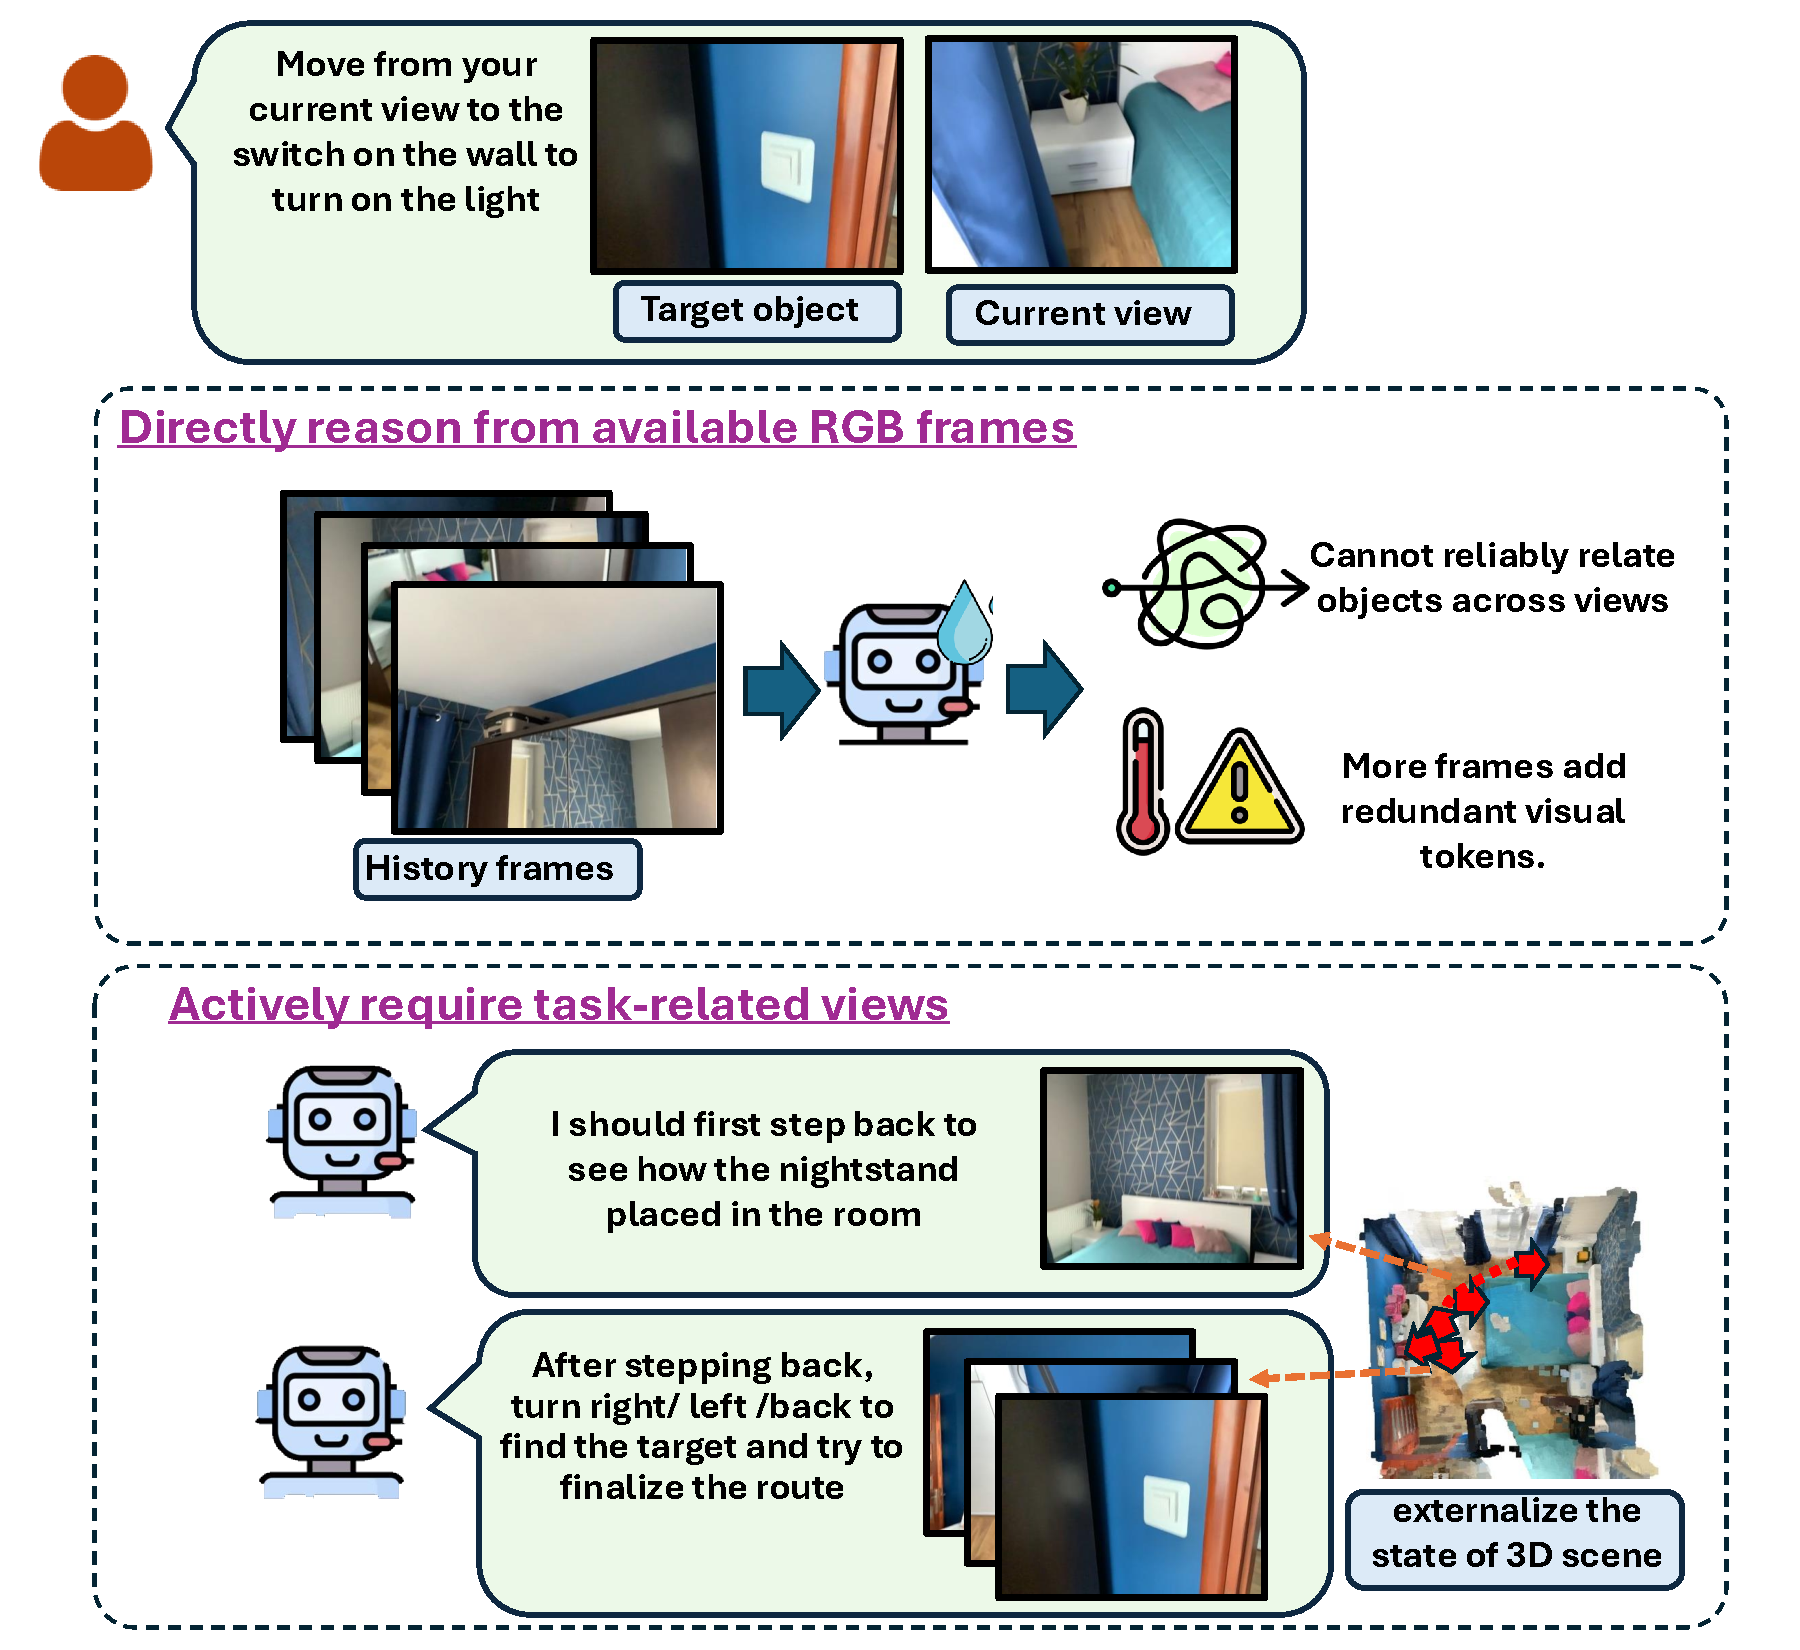
\includegraphics[width=0.85\linewidth]{figures/method_rationale.pdf}
	\vspace{-0.1in}
	\caption{ViewTree renders task-relevant views from one reconstructed scene instead of processing redundant history frames.}
	\label{fig:method_rationale}
	\vspace{-0.15in}
\end{figure}
	
	
	An intuitive solution to this deficiency of VLMs is to explicitly provide 3D information to the VLM. Existing methods inject 3D supervision during VLM training~\cite{spatialvlm2024,ross3d2025}, or construct bird's-eye-view (BEV) and semantic maps from observed frames~\cite{gpt4scene2025,mosaicthinker2026}. Although these approaches can improve spatial grounding, the fixed global representation they provide may not be always suitable for a small on-device VLM, because using dense geometry contains substantial task-irrelevant information and using a sparse map must decide in advance which objects and relationships to preserve. In both cases, the VLM passively receives a predetermined representation that may not contain all the spatial information required by VLM's reasoning.
	
	Instead, a better alternative is to externalize the state of 3D scene and allow the VLM to \emph{actively acquire} the necessary spatial information in task-related views. %For example, after observing that a cabinet occludes the queried doorway, the VLM can request a leftward camera motion. The returned view is appended to the reasoning context, and the VLM can determine whether the doorway becomes visible, request another motion, or answer. Such an action-observation loop can convert an occlusion or coordinate-transformation problem into a simpler visual comparison from a deliberately selected viewpoint.
	Rather than requesting camera movements in the physical world to capture new views that is usually infeasible in practice, recent work suggest that a VLM uses the new views generated from a \emph{world model} \cite{mindjourney2025,spatialdreamer2025,avic2026,astra2026}. 
	%The VLM first chooses a camera movement, and the world model then generates an image from the requested viewpoint. 
	Doing so can help reveal an occluded object or show a spatial relationship from a viewpoint that is easier for the VLM to perceive. \textcolor{red}{For example, as shown in Figure~\ref{fig:method_rationale}, the VLM can first request a view from farther back to locate the nightstand and then request a view facing the nearby wall to find the light switch. In this way, the VLM uses a small number of task-related views instead of reasoning over all history frames at once.} However, the generated view is only a prediction from the world model rather than an actual observation from the captured scene.
	Especially when the prediction corresponds to large camera movement, the world model's prediction may lose physical consistency and largely deviate from the actual scene \cite{visa2025}, \textcolor{red}{as shown in Figure \ref{fig:world_model_failure}}. Leveraging multiple prediction from the world model can help, but adds substantial compute cost to mobile devices.

    
    \begin{figure}
	\centering
	\vspace{-0.05in}
	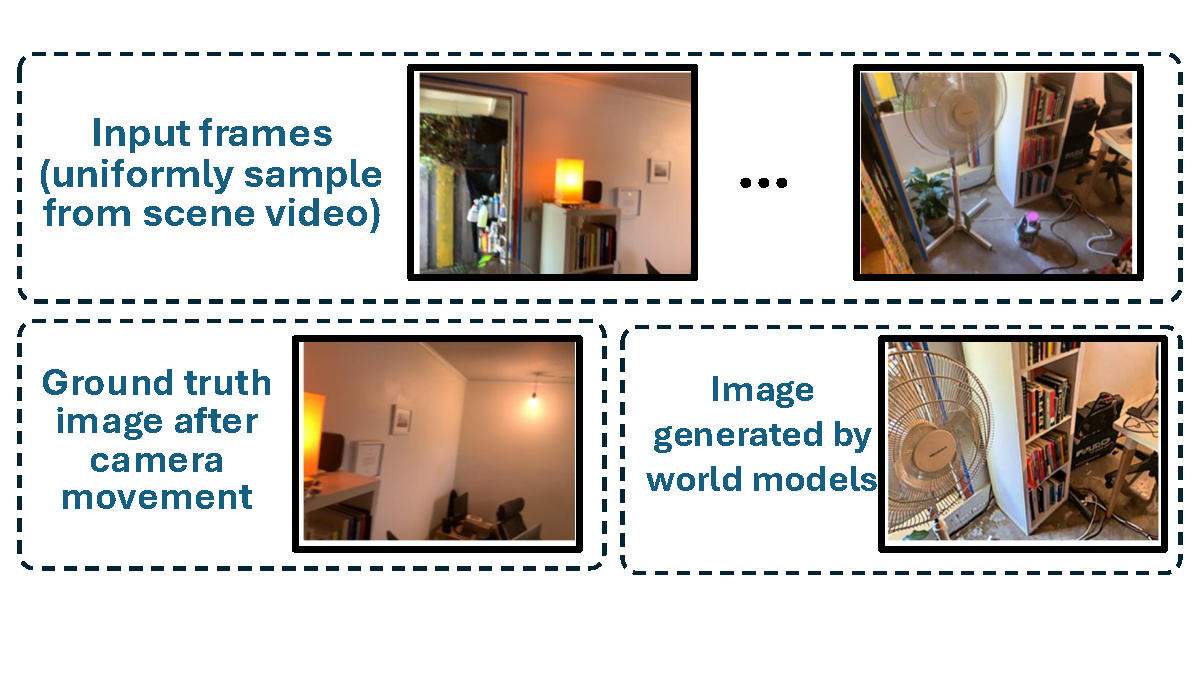
\includegraphics[width=0.85\linewidth]{figures/world_model_failure.pdf}
	\vspace{-0.1in}
	\caption{Failure mode of using world model for view prediction: physical inconsistency}
	\label{fig:world_model_failure}
	\vspace{-0.15in}
\end{figure}

	%To minimize such physical inconsistency, our basic idea, as shown in Figure ?? \textcolor{red}{[I don't understand your write-up here. Are you saying that you use one predicted view as input for another world model prediction? Use the same figure to illustrate your basic idea? if needed, you can put two subfigures there: one to show the existing work and another to show your idea]}, is to reconstruct the observed scene once and use the reconstruction to render each requested camera view, rather than generating them with a world model \textcolor{red}{[I don't understand the difference between the two, and what you mean by "reconstruct the observed scene" "use the reconstruction to render".]}. 

    \textcolor{red}{To reduce inconsistency across requested views, we use a geometry model such as VGGT~\cite{vggt2025} to reconstruct the captured scene as a set of 3D points with estimated camera poses. When the VLM selects a camera movement, the system moves a virtual camera to the requested pose and projects the stored 3D points into a new 2D view. Compared with images generated by a world model, the rendered view may contain less detailed textures or missing pixels due to limited resolution but preserves the geometry of the original scene.}

	To address the possible cascaded error propagation across predicted views, we allow a VLM to adaptively explore multiple camera paths in a reconstructed 3D scene. While an easy question can be answered from the current view or after one camera movement, a more difficult question can explore additional paths.
	
	
	%However, when several camera movements appear useful, an incorrect early choice may lead the VLM toward a region that does not contain the required information. Existing methods that follow a single reasoning path~\cite{cov2026,think3d2026} may also be insufficient when answering a question requires observations from different directions. To explore multiple paths efficiently, instead of expanding several camera paths at every reasoning step, the system must adaptively determine when alternative camera trajectories are necessary, which trajectories should receive computation, and when their observations should be combined, subject to the device’s latency, energy, memory constraints.
	
	Based on this idea, in this paper we present \system, an on-device spatial reasoning system that first uses a frozen geometry model to reconstruct recent history frames~\cite{vggt2025}, and then maintains the reconstructed scene across nearby questions to provide a virtual camera that the VLM can control. At each reasoning step, the VLM selects one of four operations: \textsc{Move}, \textsc{Branch}, \textsc{Fuse}, or \textsc{Stop}. \textsc{Move} changes the virtual camera position and returns an encoded view with its camera pose. In this way, the VLM receives only the view requested by its current reasoning, rather than processing the complete 3D reconstruction.
	
	The main challenge is to explore multiple camera paths without introducing unnecessary computation. \system adds a learned confidence head that predicts whether each partial path can eventually produce the correct answer. When the current answer has low confidence and several camera movements appear useful, the VLM can create a small number of paths from the same reasoning history. These paths reason independently so that an incorrect decision in one path does not affect the others. After each movement, \system retains paths with high confidence and removes paths with low confidence. If several high-confidence paths produce different answers, the system keeps them and requests another view that can help resolve the disagreement. Observations from different paths are combined only when they provide complementary information. If one path already answers the question with high confidence, the system stops without combining additional observations.
	
	To run efficiently on mobile devices, \system reuses computation shared by different camera paths. The 3D reconstruction is reused across nearby questions, while rendered views and visual features are cached for later requests. Camera movements from different paths are rendered and encoded in batches, and the paths share the VLM’s prefix KV cache before they separate. A device-aware scheduler adjusts the number and length of camera paths according to the available latency, energy, memory, and thermal budget. In this way, the VLM decides which paths are useful, while the scheduler determines how many useful paths the device can support.
	
	[I didn't revise the above 3 paragraphs. I will need to see your figures and revisions to fully understand these before revision.]
	
	This paper makes the following contributions:
	
	\section{Background and Motivation}
	\label{sec:background}
	\subsection{Spatial Reasoning from Fixed Views}
	Existing 3D question-answering benchmarks ask a VLM to reason from the current image, a set of history frames, or a video clip~\cite{scanqa2021,sqa3d2022,openeqa2024}. This input is sufficient when the queried objects are visible in one view. However, perspective taking, occlusion, and spatial memory often require information from a different camera position. Recent benchmarks show that current VLMs remain unreliable when the same object appears at different locations across views or when the required objects are observed in separate frames~\cite{vsibench2024,mindcube2025}.
	
	One common solution is to append more history frames. These frames come directly from the captured scene, but the VLM must still determine which frames are useful, estimate how the camera moved, and match the same objects across views. Supplying more frames also increases visual-token computation and may distract a small VLM with repeated or irrelevant observations. Other work converts the history frames into a fixed bird's-eye-view or semantic map~\cite{gpt4scene2025,mosaicthinker2026}. Such maps align information across views, but they must decide in advance which scene information to include and do not allow the VLM to request a missing view during reasoning.
	
	These limitations motivate \system to let the VLM choose what to observe next. Instead of processing a fixed number of frames or one fixed map, the VLM can request a camera movement when the current views do not provide enough information.
	
	\subsection{Generating or Rendering New Views}
	Recent work allows a VLM to request new views from a generative world model~\cite{mindjourney2025,spatialdreamer2025,avic2026,astra2026}. The VLM chooses a camera movement, and the world model generates an image from the requested viewpoint. This can reveal an occluded object or show a spatial relationship from a view that is easier to understand. However, the generated image is a prediction rather than an actual observation from the captured scene. A large camera movement may produce frames that are geometrically inconsistent with one another or with the actual scene layout~\cite{visa2025}. Generating several views also adds substantial latency and energy consumption on mobile devices.
	
	Another approach reconstructs the observed scene and renders virtual views from the reconstruction. All rendered views then refer to the same stored geometry, and rendering is less expensive than generating new scene content. However, directly providing the complete point cloud or a dense set of rendered views introduces substantial irrelevant information. A small VLM may have difficulty finding the few views needed for the current question.
	
	These limitations motivate \system to reconstruct the scene once but expose it through a virtual camera. The VLM receives only the 2D view requested by its current reasoning, while every requested view is rendered from the same reconstructed scene.
	
	\subsection{Single and Multiple Reasoning Paths}
	Existing methods allow a VLM to move a virtual camera through a reconstructed 3D scene~\cite{cov2026,think3d2026}. These methods follow one camera path. When several movements appear useful, an incorrect early choice may lead the VLM toward a region that does not contain the required information. One path may also be insufficient when answering a question requires observations from different directions. General multimodal tree-search methods can explore several reasoning paths~\cite{visuothink2025}, and fixed camera grids can render several views in advance~\cite{cdviews2025}. However, expanding many camera paths at every step is too expensive for mobile devices. Each additional path requires view rendering, visual encoding, VLM decoding, and memory for its reasoning history. More views are not always helpful because repeated or irrelevant observations may reduce the accuracy of a small VLM. These limitations motivate \system to create reasoning paths only when the input frames are insufficient. 
	
	\section{System Overview}
	\label{sec:overview}
	\begin{figure*}[t]
		\centering
		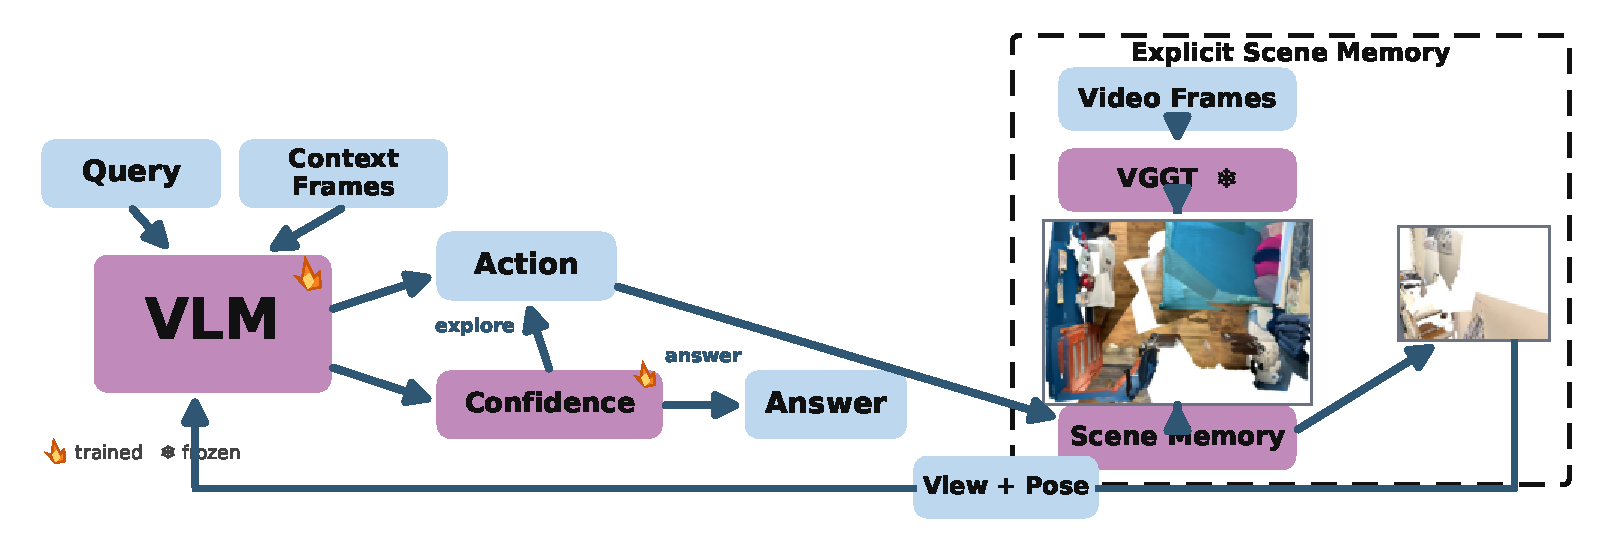
\includegraphics[width=0.97\textwidth]{figures/fig_overview.pdf}
		\vspace{-0.12in}
		\caption{\system overview on a real scene. The recent frames are reconstructed once into an explicit scene memory that can render validity-checked views from discrete camera poses (1); a learned gate answers directly when the frames suffice (2); otherwise confidence-guided camera walks acquire the missing views, stop early on agreement, and a final arbitration chooses between the direct and explored answers (3).}
		\label{fig:overview}
	\end{figure*}
	
	%Let $V=\{v_1,\ldots,v_n\}$ denote the available RGB frames and $q$ a natural-language question. Depending on the workload, $V$ contains 16--32 uniformly sampled video frames, the most recent image history, or up to four given views. We consider static indoor scenes and questions about object locations, relative directions, occlusion, containment, and navigation. If an area is not supported by the reconstruction, \system does not generate its content or treat it as observed.
	
	As shown in Figure~\ref{fig:overview}, \system contains three main components. First, confidence-guided viewpoint reasoning represents each reasoning path as a multi-step camera walk and retains several walks when the next useful movement is uncertain. Second, offline training teaches the view-conditioned answerer, camera policy, exploration gate, and confidence head. Third, the implementation reuses each scene reconstruction, caches views by camera pose, and batches rendering work. Sections~\ref{sec:reasoning}--\ref{sec:runtime} describe these components in the same order.
	
	\subsection{Online: Adaptive Viewpoint Reasoning}
	\label{sec:overview-reasoning}
	Let $V=\{v_1,\ldots,v_n\}$ denote the available RGB frames and $q$ a natural-language question. Consider a perspective-taking question whose answer is not visible from the current frames, such as asking which object is to the left of a chair when facing it from the opposite side. A useful reasoning path should first decide which change of viewpoint may reveal the relation, acquire that view, and then reconsider the question using the new observation and its camera pose. If the relation remains occluded, the reasoner should choose another movement from its new location. So the reasoning path therefore looks like
	\begin{equation}
		(q,V)\rightarrow a_1\rightarrow(o_1,p_1)
		\rightarrow a_2\rightarrow(o_2,p_2)\rightarrow y,
		\label{eq:reasoning-path}
	\end{equation}
	where every action $a_i$ produces a novel view $o_i$ at pose $p_i$ and updates the answer $y$. For some questions, several first movements are plausible. Following only one can commit the reasoner to an uninformative side of the scene. The reasoning process should be able retain several camera walks, evaluate each with its own observations, and spend later steps only on the walks that remain likely to answer correctly.
	
	To realize this process, \system first uses frozen VGGT to reconstruct the input frames into a stored 3D scene
	\begin{equation}
		\mathcal{M}=\Phi_{3D}(V),
	\end{equation}
	containing scene points, camera parameters, and visibility information. For a camera pose $p$, a point-splat renderer returns a 2D image and a geometric support mask:
	\begin{equation}
		(o_p,m_p)=\mathcal{R}(\mathcal{M},p).
		\label{eq:observe}
	\end{equation}
	%Candidate poses are restricted to locations a person holding a camera could occupy: they lie inside the recorded camera trajectory, remain at eye level with zero roll, keep clearance from reconstructed surfaces, and must render at least 45\% supported pixels. This hard constraint prevents the camera walk from moving outside the room or above the ceiling. Valid poses form a 97-pose bank, and the controller moves through it using turns, forward motion, movement to another standing position, a look-around action, a final bird's-eye view, or \textsc{Stop}. Every rendered image is paired with a text tag describing its standing position and viewing direction.
	
	\system begins by answering from the input frames and deciding whether exploration is necessary. If so, each active reasoning path proposes camera actions. Beam search expands the three actions with the largest controller probabilities and uses a calibrated confidence head to retain the two most promising resulting states. Each retained path keeps its own sequence of actions, poses, rendered observations, and answers. Search continues for at most three acquired views. It can stop earlier when the retained paths agree with sufficient confidence; otherwise, final arbitration compares the best explored state with the original direct answer. Thus, \system implements the desired action--observation reasoning loop without requiring the VLM to process the complete 3D reconstruction. Section~\ref{sec:reasoning} gives the state, action, pruning, and stopping rules.
	
	\subsection{Offline: Reasoning Policy Training}
	\label{sec:overview-training}
	ViewTree must learn four abilities: answer from the available views, decide whether another view is needed, choose where the camera should move, and estimate whether the current answer is reliable. We train these abilities in three SFT stages and a reinforcement-learning stage.
	
	First, we train the VLM to answer from rendered views. The input contains the question, the original frames, and zero or more rendered views with their camera poses. Examples without rendered views teach the VLM to answer directly when the original frames are sufficient.
	
	Second, we train the VLM to control the virtual camera. During training, the system tries camera movements that satisfy the physical constraints and checks whether the resulting views lead to the correct answer. It then selects the shortest successful viewpoint trajectory whose answer exceeds the required confidence margin. If the direct answer is already correct, the target action is \textsc{Stop}. This teaches the controller to avoid unnecessary exploration. We refer to this trial-and-check procedure as oracle search.
	
	Third, we train the confidence head. Each partial viewpoint trajectory visited during oracle search is labelled according to whether the answer produced from that trajectory is correct. The confidence head learns to predict this outcome from the VLM's internal state and is calibrated on held-out scenes. During inference, ViewTree uses this score to retain promising paths and remove weak ones. Search stops when the retained paths agree on an answer with higher confidence than the direct answer. Final arbitration then selects the highest-confidence answer among the direct and explored answers.
	
	Finally, we optionally apply reinforcement learning over complete viewpoint trajectories while penalizing additional camera steps. In our experiments, this stage improved answer prediction but did not improve camera-action selection. The final system therefore uses the controller trained from oracle trajectories.
	
	\subsection{System Execution}
	\label{sec:overview-runtime}
	ViewTree repeatedly queries the same reconstructed scene while exploring different camera paths. To avoid repeated work, the system reconstructs each scene once and reuses the resulting world memory across questions and paths. Rendered views are cached by camera pose, and views requested at the same search level are rendered together. The current implementation processes the resulting VLM states sequentially.
	
	ViewTree bounds the cost of camera exploration through the exploration gate, fixed search limits, and early stopping. It also removes camera actions whose target views are not sufficiently supported by the reconstruction. Section~\ref{sec:runtime} presents the runtime design -- reconstruction reuse, view and token caching, batched and decode-free search steps, and bounded search -- together with its measured latency, energy, and memory on an embodied device.
	
	\section{Online: Adaptive Viewpoint Reasoning}
	\label{sec:reasoning}
	As described in Section~\ref{sec:overview-reasoning}, \system organizes viewpoint acquisition as confidence-guided search over multi-step viewpoint trajectory. This section describes the reasoning state, valid camera actions, exploration gate, beam expansion, pruning, and stopping rules.
	
	\subsection{Viewpoint State and Action Space}
	
	Instead of providing the complete 3D scene memory to the VLM, the reasoning path in \system contains only the information needed to select the next viewpoint and update the answer: the question, the original frames, the rendered views acquired so far, and a short textual pose tag for each view that tells the VLM where the camera was standing and which way it was facing when the view was captured. The complete 3D scene never enters the VLM's input context, so the context length grows with the handful of acquired views rather than with the scene.

\begin{figure}[t]
	\centering
	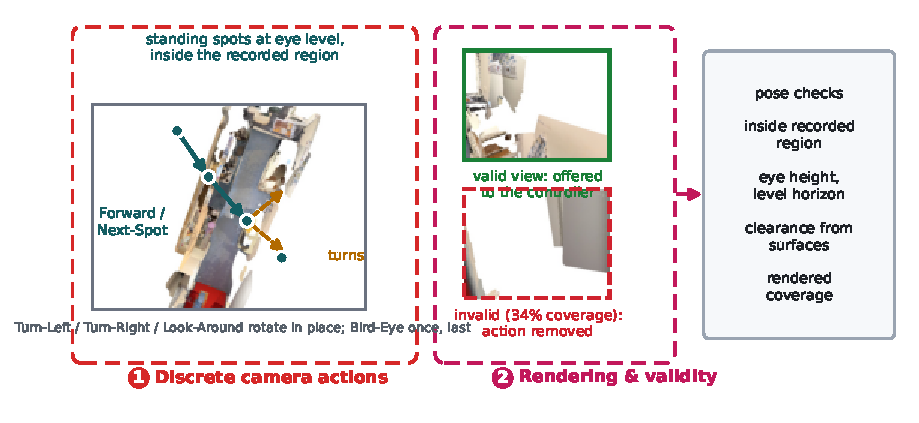
\includegraphics[width=\linewidth]{figures/fig_action_space.pdf}
	\vspace{-0.25in}
	\caption{Camera actions and pose validity on a real reconstructed scene. The virtual camera moves between discrete standing spots and viewing directions (left); each candidate pose is rendered and checked before it is offered to the controller (middle, right).}
	\label{fig:action_space}
	\vspace{-0.15in}
\end{figure}

	As shown in Figure~\ref{fig:action_space}, \system exposes the scene memory through a small set of camera actions rather than free 3D coordinates: \textsc{Turn-Left} and \textsc{Turn-Right} rotate the view in place, \textsc{Forward} moves to a nearby standing position along the current direction, \textsc{Next-Spot} jumps to another valid standing position, \textsc{Look-Around} turns to the opposite direction, \textsc{Bird-Eye} requests a single top-down view as the final acquisition, and \textsc{Stop} ends the trajectory. Discrete actions keep three things simple at once: the training-time search over alternatives (Section~\ref{sec:training}) only needs to enumerate a handful of successors per state; the controller emits an action as a single token instead of numeric coordinates; and every pose maps to a small cache key, which the runtime exploits heavily (Section~\ref{sec:runtime}).

	Before the controller selects an action, \system checks whether the resulting pose is physically plausible and renderable: the pose must stay inside the region the camera actually recorded, keep the camera at eye height with a level horizon, maintain clearance from reconstructed surfaces, and produce a rendering with sufficient geometric support (Figure~\ref{fig:action_space}, right). Actions that fail these checks are removed from the controller's choices. The controller therefore chooses only among views that can be reliably rendered, rather than having to learn to avoid unsupported poses from training examples.

	\subsection{Deciding When to Explore}
	\label{sec:confidence}
	Not every question requires a new viewpoint. When the original frames already contain the answer, rendering additional views adds unnecessary computation and may introduce irrelevant or incomplete visual information that reduces answer accuracy. \system therefore first produces a direct answer from the original frames and, in the same breath, asks the model a single learned gating question: do these frames alone contain enough information to answer? If the gate answers \textsc{Yes}, the direct answer is returned immediately after only two short VLM calls; across our evaluation this happens on 71\% of questions. Only when the gate answers \textsc{Explore} does \system start the search: the camera controller scores the actions allowed at the current pose, and beam search creates alternative reasoning paths from the highest-scoring ones. The gate decides whether a search tree is needed at all, while the controller decides how each path should move through the scene. Figure~\ref{fig:gate_example} shows both outcomes on real questions.

\begin{figure}[t]
	\centering
	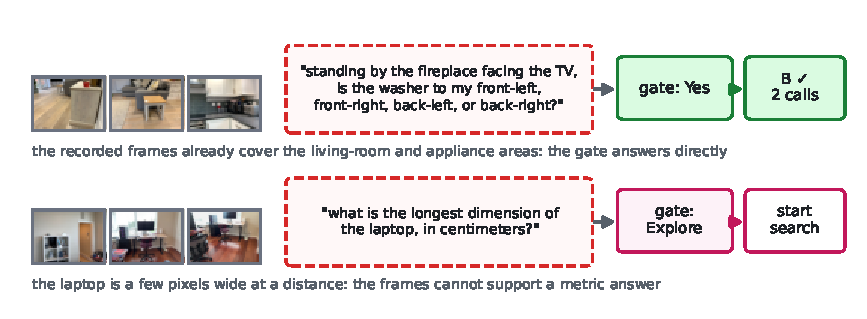
\includegraphics[width=\linewidth]{figures/fig_gate_example.pdf}
	\vspace{-0.25in}
	\caption{The exploration gate on two real questions. Top: the frames cover the queried areas, so the direct answer is returned after two calls. Bottom: the object's size cannot be judged from distant frames, so the gate starts the search.}
	\label{fig:gate_example}
	\vspace{-0.15in}
\end{figure}

	\subsection{Confidence-Guided Path Expansion and Pruning}
	Figure~\ref{fig:control_prompt} shows one controller step. The controller receives the context frames, the views acquired so far with their pose tags, the question, and the list of currently valid moves, and replies with exactly one action token. \system reads the scores of all valid actions directly from this single forward pass, expands the three highest-scoring actions, and creates a separate successor path for each: a movement action renders the new view and asks the VLM for an updated answer, while \textsc{Stop} marks the path as terminal without another render.

\begin{figure}[t]
	\centering
	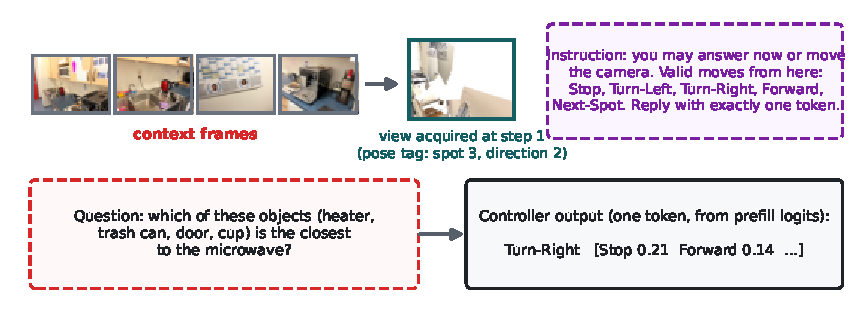
\includegraphics[width=\linewidth]{figures/fig_control_prompt.pdf}
	\vspace{-0.25in}
	\caption{One camera-controller step. The valid moves are listed in the prompt, and the scores of all candidate actions are read from a single prefill pass, so a control step costs no answer decoding.}
	\label{fig:control_prompt}
	\vspace{-0.15in}
\end{figure}

	Each successor also needs a score that says how promising it is. Verbalized self-confidence and answer-token probability are known to be poorly calibrated for this purpose; instead, a small two-layer head reads the VLM's last-token hidden state $\bar{h}_b$ at the answer and predicts the probability that this answer is correct:
\begin{equation}
	c_b=\sigma\!\left(\operatorname{MLP}(\bar{h}_b)/T\right),
	\label{eq:confidence}
\end{equation}
where the temperature $T$ is fitted on held-out scenes. The head is trained on the outcomes of training-time search (Section~\ref{sec:training}), so its scores are comparable across paths and depths. After expanding all active paths, \system simply keeps the two successors with the highest calibrated confidence. Retained paths share the question and context frames, but their acquired views and later reasoning remain separate, so one early wrong turn cannot contaminate a sibling path.

	\subsection{Path Stopping and Final Answer Selection}
	\label{sec:path-evidence}
	Views are accumulated within each camera walk rather than combined across sibling paths: at every step, the VLM of a path sees the original frames followed by that path's views in acquisition order, each preceded by its pose tag. The ordered tags tell the VLM how the camera moved, which lets a later step reuse evidence collected earlier along the same walk. Figure~\ref{fig:search_example} traces a real \system search: the retained paths approach the queried objects from different directions and converge on the same answer at depth three.

\begin{figure}[t]
	\centering
	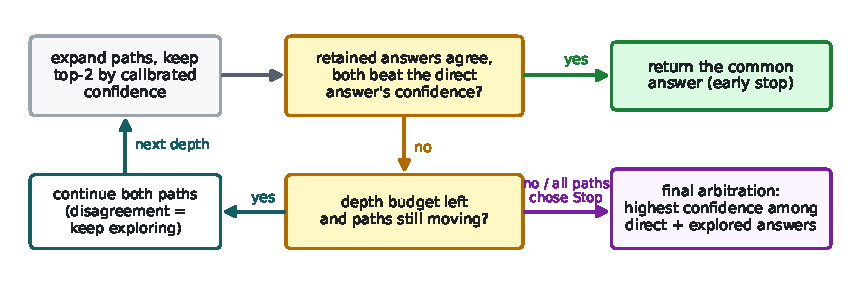
\includegraphics[width=\linewidth]{figures/fig_stopping.pdf}
	\vspace{-0.28in}
	\caption{How a search ends: early stop on confident agreement, deeper exploration on disagreement, and final arbitration otherwise.}
	\label{fig:stopping}
	\vspace{-0.15in}
\end{figure}

	The search stops in one of three ways (Figure~\ref{fig:stopping}). If the two retained paths agree on the same answer and both are more confident than the direct answer, \system stops early and returns the common answer -- agreement between independently moving paths is strong evidence. If they disagree and depth remains, both paths continue so that their next camera actions can collect discriminating evidence. Otherwise, at the depth limit or when all retained paths choose \textsc{Stop}, \system compares the calibrated confidence of the direct answer and of the retained explored answers, and returns the highest-scoring one:
\begin{equation}
	\hat{y}=y_{k^{*}},\qquad
	k^{*}=\arg\max_{k\in\{0\}\cup\mathcal{B}_{\mathrm{final}}}c_k,
	\label{eq:arbitration}
\end{equation}
where $k=0$ denotes the direct answer and $\mathcal{B}_{\mathrm{final}}$ the retained explored states. This final arbitration matters in practice: it prevents an incomplete or distracting reconstruction from automatically overriding an answer that was already well supported by the original frames.

\begin{figure*}[t]
	\centering
	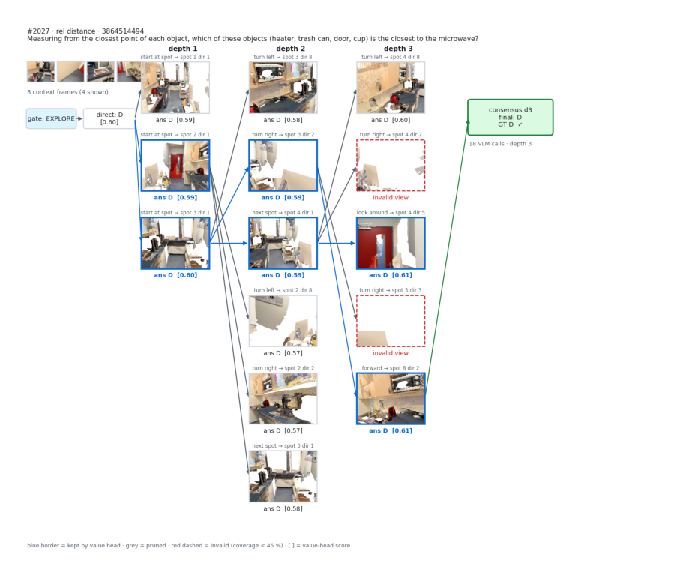
\includegraphics[width=0.92\textwidth]{figures/fig_search_example.pdf}
	\vspace{-0.15in}
	\caption{A real \system search on a VSI-Bench question. The gate finds the frames insufficient; the beam explores three standing spots, prunes by calibrated confidence (blue borders), discards views without geometric support (red dashed), and stops at depth three when the retained paths agree on the correct answer.}
	\label{fig:search_example}
	\vspace{-0.1in}
\end{figure*}

		Algorithm~\ref{alg:viewtree} summarizes \system inference.
	%\subsection{Reasoning under an Acquisition Budget}
	%Algorithm~\ref{alg:viewtree} summarizes \system inference. We use action expansion width three, beam width two, and maximum depth three. The controller can stop a path before the depth limit, while the initial gate avoids the tree entirely when the context frames are sufficient. These fixed limits replace the unimplemented live device scheduler.
	
	\begin{algorithm}[t]
		\caption{Confidence-guided ViewTree inference}
		\label{alg:viewtree}
		\begin{algorithmic}[1]
			\Require Question $q$, frames $V$, memory $\mathcal{M}$
			\Ensure Answer $y$
			\State $(y_0,c_0,g)\gets\textsc{DirectAnswerAndGate}(q,V)$
			\If{$g=\textsc{Yes}$}
			\State \Return $y_0$
			\EndIf
			\State $\mathcal{B}\gets\{\textsc{Init}(q,V)\}$
			\For{$i=0$ to $D-1$}
			\State $\widetilde{\mathcal{B}}\gets\emptyset$
			\ForAll{$b\in\mathcal{B}$}
			\State $A_b\gets\textsc{TopValidActions}(b,3)$
			\ForAll{$a\in A_b$}
			\If{$a=\textsc{Stop}$}
			\State $\widetilde{\mathcal{B}}\gets
			\widetilde{\mathcal{B}}\cup\{\textsc{Terminal}(b)\}$
			\Else
			\State $b'\gets\textsc{Observe}(b,a,\mathcal{M})$
			\State $\widetilde{\mathcal{B}}\gets
			\widetilde{\mathcal{B}}\cup\{b'\}$
			\EndIf
			\EndFor
			\EndFor
			\State $\mathcal{B}\gets\textsc{TopK}(\widetilde{\mathcal{B}},c,2)$
			\If{$\textsc{ConfidentAgreement}(\mathcal{B},c_0)$}
			\State \Return common answer of $\mathcal{B}$
			\EndIf
			\EndFor
			\State \Return highest-confidence answer in $\{y_0\}\cup\mathcal{B}$
		\end{algorithmic}
	\end{algorithm}
	
	With these settings, a gated question uses two VLM calls. Across the evaluation, \system uses 4.5 calls per question on average; a full depth-three search can require approximately 20 answer and action-proposal calls, but such deep searches are rare (8\% of questions). Because the gated calls are short, the common case is cheap: on the embodied device, the two-call gated route finishes faster than a single 16-frame direct-input call (Section~\ref{sec:runtime}). We therefore report calls, renders, and acquired views in addition to accuracy.
	
	\section{Offline Reasoning-Policy Training}
	\label{sec:training}
	
	ViewTree must learn four abilities: answer from the available views, decide whether another view is needed, select where the virtual camera should move, and estimate whether the current answer is reliable. As shown in Figure~\ref{fig:training_pipeline}, we train these abilities in three stages, followed by an optional reinforcement-learning stage.

\begin{figure}[t]
	\centering
	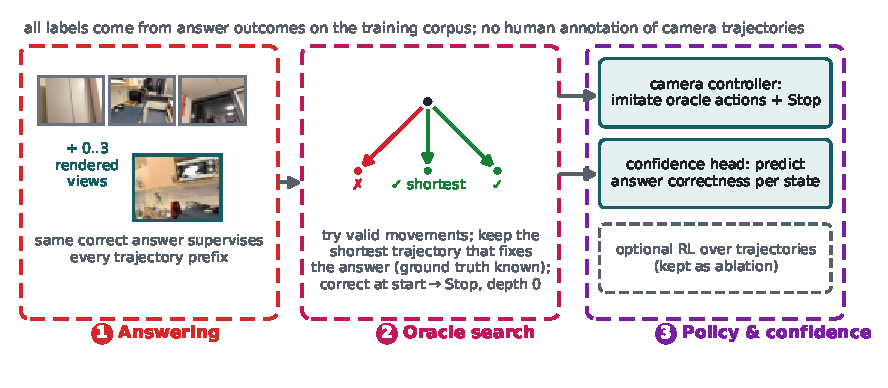
\includegraphics[width=\linewidth]{figures/fig_training_pipeline.pdf}
	\vspace{-0.25in}
	\caption{\system training. The answerer is first taught to use rendered views (stage 1); a training-time oracle search discovers which camera trajectories fix wrong answers (stage 2); its actions and visited states then supervise the camera controller and the confidence head (stage 3).}
	\label{fig:training_pipeline}
	\vspace{-0.15in}
\end{figure} We first teach the VLM to answer from the original frames and newly rendered views. We then use oracle search to produce camera-action and stopping targets. Finally, we use the states visited during oracle search to train the confidence head. The optional reinforcement-learning stage improves answer prediction but not camera control in our experiments; therefore, the final system uses the controller trained from oracle trajectories.
	
	\subsection{Learning to Answer from New Views}
	
	The VLM must answer using either the original frames alone or the original frames together with newly rendered views. We therefore train it with examples taken from different steps of a camera trajectory. Each example contains the question, the original frames, the rendered views obtained so far, and the correct answer. Each rendered view is also paired with its camera location and viewing direction so that the VLM knows where the view was captured.
	
	The VLM is trained with standard next-token prediction on the answer tokens, conditioned on the question, the original frames, and the rendered views obtained so far. The same correct answer supervises every prefix of a trajectory. Some training examples contain no rendered views; these teach the VLM to answer directly when the original frames provide enough information. Other examples contain one or more rendered views and teach the VLM to revise its answer when new information arrives.

	\subsection{Finding Useful Viewpoint Trajectories}
	
	The correct answer alone does not tell the controller where to move the virtual camera. We therefore use a training-time search procedure to find useful camera trajectories. The search starts from the original camera view and tries camera movements that satisfy the physical constraints. After each movement, the system renders the resulting view and asks the VLM to answer the question again. Because the correct answer is known during training, the system can check whether each camera trajectory helps the VLM produce the correct answer.
	
	Concretely, an answer counts as correct when its evaluation score (exact match for multiple choice, relative accuracy for numerical answers) exceeds one half. If the VLM already answers correctly from the original frames, the selected trajectory is empty and the target action is \textsc{Stop}; these depth-zero examples are the most frequent labels and are what teach the controller not to over-explore. Otherwise, let $\mathcal{T}^{+}(q)$ contain the tested trajectories whose final answer is correct; the search keeps the shortest one, breaking ties by the answer margin $\operatorname{m}(\tau)$, i.e., how strongly the VLM favors the correct answer at the end (Figure~\ref{fig:training_pipeline}, middle):
\begin{equation}
	\tau^{*}=\arg\max_{\tau\in\mathcal{T}^{+}(q),\;|\tau|=\min_{\tau'\in\mathcal{T}^{+}(q)}|\tau'|}\operatorname{m}(\tau).
	\label{eq:selected-trajectory}
\end{equation} Preferring the shortest successful trajectory bakes the acquisition cost into the supervision itself: the controller is never shown a longer walk when a shorter one suffices. Figure~\ref{fig:oracle_example} walks through one oracle trajectory.

\begin{figure}[t]
	\centering
	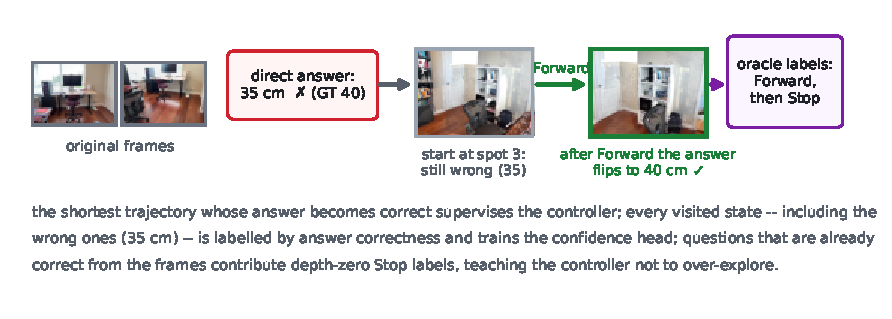
\includegraphics[width=\linewidth]{figures/fig_oracle_example.pdf}
	\vspace{-0.25in}
	\caption{An oracle trajectory on a real training question. The direct answer is wrong; one \textsc{Forward} movement fixes it, so the controller's targets are \textsc{Forward} then \textsc{Stop}, and every visited state is labelled by answer correctness for the confidence head.}
	\label{fig:oracle_example}
	\vspace{-0.15in}
\end{figure}

	The selected trajectory provides training examples for the camera controller. At each step, the views obtained so far form the controller input, and the next camera movement is used as the target action. After the final view, the target action is \textsc{Stop}. The search also keeps the states that produce incorrect answers, which are later used to train the confidence head.
	
	\subsection{Learning When and Where to Explore}
	
	The selected oracle trajectory teaches the controller both where to move and when to stop: at every prefix $h_i$ of the trajectory the controller imitates the next oracle action $a_i^{*}$, and at the final state it imitates \textsc{Stop}:
\begin{equation}
	\mathcal{L}_{\mathrm{ctrl}}=-\sum_{i=0}^{|\tau^{*}|}\log\pi_{\theta}\!\left(a_i^{*}\mid h_i\right),\qquad
	a^{*}_{|\tau^{*}|}=\textsc{Stop}.
	\label{eq:ctrl}
\end{equation} Invalid movements are removed before action prediction, so the controller only ever chooses among camera actions that can actually be executed from the current pose.

	Before rendering a new view, ViewTree prompts the controller to choose between \textsc{Yes} and \textsc{Explore}. This decision reuses the controller's learned stopping behavior and does not require a separate exploration classifier. \textsc{Yes} returns the direct answer, whereas \textsc{Explore} starts viewpoint-trajectory search. This initial decision determines whether another view is needed, while the subsequent controller decisions determine where the virtual camera should move.
	
	\subsection{Learning Confidence for Path Selection}
	
	During inference, ViewTree cannot compare a candidate answer with the ground truth. It must instead estimate which partial trajectory is likely to produce a correct answer. We therefore label every state visited during oracle search -- including the many unsuccessful ones -- by whether the answer produced at that state was correct, and train a small head on the VLM's internal state to predict this outcome. The predicted probability is calibrated on held-out scenes before it is used by the search~\cite{guo2017calibration}.

	Unlike verbal confidence or answer-token probability, $c_b$ is learned from the observed successes and failures of partial viewpoint trajectories. During inference, ViewTree uses it to rank candidate paths, retain the most promising paths, and remove weak paths. The search can stop when the retained paths agree on an answer whose confidence is higher than that of the direct answer. After exploration, ViewTree compares the direct and explored answers and returns the one with the highest calibrated confidence.
	
	\subsection{Reinforcement Learning}
	
	After supervised training, we optionally apply group-relative policy optimization to complete viewpoint trajectories~\cite{deepseekmath2024}. The reward favors correct answers while penalizing additional or invalid camera movements. This objective encourages the model to improve its answer using as few rendered views as possible.
	
	In our experiments, reinforcement learning improves answer prediction but does not improve camera-action selection. The final ViewTree system therefore uses the controller trained through imitation of the oracle trajectories. We retain the reinforcement-learned controller only as an ablation.
	
	\section{System Execution}
	\label{sec:runtime}
	ViewTree repeatedly queries the same reconstructed scene while exploring different camera paths. A direct implementation would reconstruct the scene for every question, render the same pose more than once, allow the number of candidate paths to grow with search depth, and pay a full VLM decoding pass for every control decision. Our runtime avoids all four costs (Figure~\ref{fig:runtime}). The numbers below are measured on Jetson AGX Orin (64\,GB, JetPack~6, MAXN power mode) with the 7B backbone in bf16; Section~\ref{sec:evaluation} reports the other backbones.

\begin{figure}[t]
	\centering
	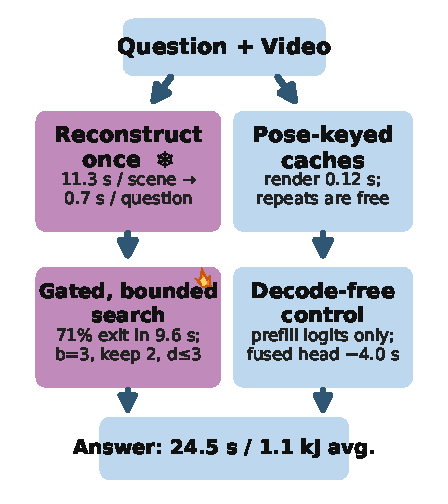
\includegraphics[width=\linewidth]{figures/fig_runtime.pdf}
	\vspace{-0.25in}
	\caption{\system runtime on the embodied device: the reconstruction is reused across questions and paths, repeated views are served from pose-keyed caches, control decisions decode nothing, and the search is bounded with a cheap gated exit.}
	\label{fig:runtime}
	\vspace{-0.15in}
\end{figure}

	\noindent\textbf{Scene reuse and view caching.} The scene memory is built once per scene and shared by every question and every search path: a 32-frame reconstruction takes 11.3\,s warm on the device, which amortizes to 0.7\,s and 32\,J per question at the benchmark's average of 18 questions per scene. Because camera poses are discrete (Section~\ref{sec:reasoning}), every rendered view and its encoded visual tokens are cached under a small pose key; a repeated request -- common when sibling paths converge on the same viewpoint -- skips both the renderer and the visual encoder. A cold render itself costs only 0.12\,s, two orders of magnitude below a VLM call, so the pipeline's cost is dominated by the VLM.

	\noindent\textbf{Batched, decode-free search steps.} Views requested by sibling paths at the same search level are rendered in one pass and encoded as one batch, avoiding per-view model switching. Two further optimizations exploit how the VLM is invoked. First, the controller's action choice is read from the logits of a single prefill pass over the listed valid moves (Figure~\ref{fig:control_prompt}), so a control step decodes nothing and costs the same 4.3\,s as the short gate call. Second, the confidence head reads the VLM's internal state directly from the answer call instead of issuing a separate scoring pass, which saves a measured 4.0\,s per scored answer. On this hardware, prefill dominates VLM latency (about 1.9\,s per thousand prompt tokens versus 0.11\,s per decoded token), which is why \system keeps its calls short -- eight context frames plus a few renders -- rather than feeding long frame sequences.

	\noindent\textbf{Bounded search under a device budget.} The search uses fixed limits -- expansion width three, two retained paths, depth at most three -- and the gate exits after two short calls on 71\% of questions. The expected cost at the measured route mix is 4.7 VLM calls, 24.5\,s, and 1{,}104\,J per question: about $2.1\times$ a single 16-frame direct-input call (11.7\,s, 529\,J), and $1.9\times$ \emph{cheaper} than a depth-one tree that renders all five candidate views for most questions (46.3\,s, 2{,}110\,J). Notably, the 71\%-frequency gated route alone (9.6\,s) is cheaper than the single direct-input call, because two short-prefill calls beat one long-prefill call. The alternative of simply adding frames scales poorly: the direct-input baseline grows superlinearly to 300\,s at 384 frames and exhausts the device memory at 512 frames, while \system's entire adaptive exploration costs roughly what five extra context frames would. Peak memory with both the VLM and the reconstruction model resident is 25.9\,GB, leaving ample headroom on the 64\,GB device for the 7B backbone; the 32B backbone fits with 4-bit weights.

	\section{Experiment Settings}
\label{sec:experiment_setting}

We evaluate ViewTree both on a server testbed and on an embodied AI device. All controller training and large-scale benchmark evaluations run on a server with 8$\times$NVIDIA H100 GPUs; the complete inference pipeline is additionally deployed on an NVIDIA Jetson AGX Orin (64\,GB) to characterize on-device feasibility. We apply VLM backbones with various parameter sizes to match different device budgets: Qwen2.5-VL-3B, Qwen2.5-VL-7B, and Qwen2.5-VL-32B \cite{bai2025qwen2}, where the 32B model is deployed on Jetson with 4-bit weight quantization.

\noindent\textbf{System setup.} On the server, all models run in PyTorch with bfloat16 precision. On Jetson AGX Orin, the VLM runs with quantized weights, and the remaining pipeline stages are executed as stage-level batches: the frozen VGGT \cite{wang2025vggt} reconstruction is computed once per scene and reused across all questions and reasoning branches; candidate views proposed at the same tree level are rendered in one point-splat pass and encoded as one batch; rendered views and their encoded tokens are cached by camera pose and scene version, so repeated requests skip both the renderer and the visual encoder. The end-to-end latency reported in Section~\ref{sec:evaluation} includes reconstruction (amortized and upfront), rendering, visual encoding, and all VLM calls of the reasoning tree.

\noindent\textbf{Benchmarks.} Our experiments evaluate the spatial-cognition capabilities that ViewTree is designed to improve. Following the task grouping of Section~\ref{sec:experiment_setting}, we use \emph{Metric Measurement} (absolute distance, object size, room size), \emph{Perspective-dependent Reasoning} (relative direction, relative distance, object counting, route planning), and \emph{Spatiotemporal Tracking} (appearance order, camera-motion and camera--object relations). We evaluate on four benchmark datasets (\textcolor{red}{()}):
\begin{itemize}
    \item \textbf{VSI-Bench \cite{yang2025thinking}} contains $>$5{,}000 QA pairs from 288 indoor videos over 10 spatial tasks; we report absolute distance (A.D.), object size (O.S.), relative distance (R.Dt.), relative direction (R.Dr.), object count (O.C.), and appearance order (Ap.Or.). To prevent any information leakage from confidence-head fitting, all VSI-Bench numbers are reported on a held-out half of the scenes (144 scenes, 2{,}557 questions) that is never touched by any training or calibration; splits are at scene level throughout.
    \item \textbf{STI-Bench \cite{li2025sti}} contains 300 videos and $>$2{,}000 QA pairs; we report dimensional measurement (D.Meas.) and 3D video grounding (Grd.) to complement VSI-Bench.
    \item \textbf{VSTI-Bench \cite{vstibench2026}} contains 5{,}736 QA pairs on ScanNet validation videos over 9 spatio-temporal types; we report the camera--object relation (C.O.) and object--object relation (O.O.) groups.
    \item \textbf{OST-Bench \cite{ostbench2025}} contains 5{,}557 multiple-choice questions probing online spatio-temporal reasoning over an agent's cumulative image history; we report the overall accuracy (Ovr.).
\end{itemize}
QA performance is evaluated as the percentage of correct answer choices; numerical tasks (absolute distance, object size, room size, and the numerical VSTI types) use Mean Relative Accuracy.

\noindent\textbf{Baselines.} We compare ViewTree against the following baselines, all using the same VLM backbone, visual resolution, frame budgets, and answer scorer:
\begin{itemize}
    \item \textbf{Direct input} uniformly downsamples the video and feeds the frames directly to the VLM.
    \item \textbf{Standard SFT} 
    \item \textbf{Standard SFT+GRPO} further applies GRPO with answer-correctness reward on top of standard SFT.
    \item \textbf{Video-COT}
    \item \textbf{Static Scene memory} 
\end{itemize}


\noindent\textbf{Training setup.} 

% ===================================================================
\section{Performance Evaluation}
\label{sec:evaluation}

\subsection{Spatial Task Performance}
\label{sec:main_results}

We conducted comprehensive evaluations over the spatial cognition tasks, with VLM backbones of different parameter sizes. Results in Tables~\ref{tab:vt_main_3B}--\ref{tab:vt_main_32B} show that ViewTree enhances 

% ------------------------------------------------------------------
\begin{table*}[h!]
	\centering
	\resizebox{\textwidth}{!}{%
		\begin{tabular}{lccccccccccccc}
			\toprule
			\multirow{2}{*}{\textbf{Method}} & \multicolumn{7}{c}{\textbf{VSI-Bench (held-out)}} & \multicolumn{3}{c}{\textbf{STI-Bench}} & \multicolumn{2}{c}{\textbf{VSTI-Bench}} & \textbf{OST} \\
			\cmidrule(lr){2-8} \cmidrule(lr){9-11} \cmidrule(lr){12-13} \cmidrule(lr){14-14}
			& A.D. & O.S. & R.Dt. & R.Dr. & O.C. & Ap.Or. & \textbf{Avg} & D.Meas. & Grd. & \textbf{Avg.} & C.O. & O.O. & Ovr. \\
			\midrule
			Direct Input                 & -- & -- & -- & -- & -- & -- & -- & -- & -- & -- & -- & -- & -- \\
			SFT-plain                    & -- & -- & -- & -- & -- & -- & -- & -- & -- & -- & -- & -- & -- \\
			SFT+GRPO-plain               & -- & -- & -- & -- & -- & -- & -- & -- & -- & -- & -- & -- & -- \\
			Static memory                & -- & -- & -- & -- & -- & -- & -- & -- & -- & -- & -- & -- & -- \\
			Video-COT            & -- & -- & -- & -- & -- & -- & -- & -- & -- & -- & -- & -- & -- \\
			\textbf{ViewTree}          & -- & -- & -- & -- & -- & -- & -- & -- & -- & -- & -- & -- & -- \\

			\bottomrule
		\end{tabular}
	}
	\caption{Performance with Qwen2.5-VL-3B. Task acronyms are defined in Section~\ref{sec:experiment_setting}.}
	\vspace{-0.2in}
	\label{tab:vt_main_3B}
\end{table*}

\begin{table*}[h!]
	\centering
	\resizebox{\textwidth}{!}{%
		\begin{tabular}{lccccccccccccc}
			\toprule
			\multirow{2}{*}{\textbf{Method}} & \multicolumn{7}{c}{\textbf{VSI-Bench (held-out)}} & \multicolumn{3}{c}{\textbf{STI-Bench}} & \multicolumn{2}{c}{\textbf{VSTI-Bench}} & \textbf{OST} \\
			\cmidrule(lr){2-8} \cmidrule(lr){9-11} \cmidrule(lr){12-13} \cmidrule(lr){14-14}
			& A.D. & O.S. & R.Dt. & R.Dr. & O.C. & Ap.Or. & \textbf{Avg} & D.Meas. & Grd. & \textbf{Avg.} & C.O. & O.O. & Ovr. \\
			\midrule
			Direct Input                 & -- & -- & -- & -- & -- & -- & -- & -- & -- & -- & -- & -- & -- \\
			SFT-plain                    & -- & -- & -- & -- & -- & -- & -- & -- & -- & -- & -- & -- & -- \\
			SFT+GRPO-plain               & -- & -- & -- & -- & -- & -- & -- & -- & -- & -- & -- & -- & -- \\
			Static memory                & -- & -- & -- & -- & -- & -- & -- & -- & -- & -- & -- & -- & -- \\
			Video-COT           & -- & -- & -- & -- & -- & -- & -- & -- & -- & -- & -- & -- & -- \\
			\textbf{ViewTree}          & -- & -- & -- & -- & -- & -- & -- & -- & -- & -- & -- & -- & -- \\
			\bottomrule
		\end{tabular}
	}
	\caption{Performance with Qwen2.5-VL-7B. Task acronyms are defined in Section~\ref{sec:experiment_setting}.}
	\vspace{-0.2in}
	\label{tab:vt_main_7B}
\end{table*}

\begin{table*}[h!]
	\centering
	\resizebox{\textwidth}{!}{%
		\begin{tabular}{lccccccccccccc}
			\toprule
			\multirow{2}{*}{\textbf{Method}} & \multicolumn{7}{c}{\textbf{VSI-Bench (held-out)}} & \multicolumn{3}{c}{\textbf{STI-Bench}} & \multicolumn{2}{c}{\textbf{VSTI-Bench}} & \textbf{OST} \\
			\cmidrule(lr){2-8} \cmidrule(lr){9-11} \cmidrule(lr){12-13} \cmidrule(lr){14-14}
			& A.D. & O.S. & R.Dt. & R.Dr. & O.C. & Ap.Or. & \textbf{Avg} & D.Meas. & Grd. & \textbf{Avg.} & C.O. & O.O. & Ovr. \\
			\midrule
			Direct Input                 & -- & -- & -- & -- & -- & -- & -- & -- & -- & -- & -- & -- & -- \\
			SFT-plain                    & -- & -- & -- & -- & -- & -- & -- & -- & -- & -- & -- & -- & -- \\
			SFT+GRPO-plain               & -- & -- & -- & -- & -- & -- & -- & -- & -- & -- & -- & -- & -- \\
			Static memory                & -- & -- & -- & -- & -- & -- & -- & -- & -- & -- & -- & -- & -- \\
			Video-COT            & -- & -- & -- & -- & -- & -- & -- & -- & -- & -- & -- & -- & -- \\
			\textbf{ViewTree}          & -- & -- & -- & -- & -- & -- & -- & -- & -- & -- & -- & -- & -- \\
			\bottomrule
		\end{tabular}
	}
	\caption{Performance with Qwen2.5-VL-32B (4-bit on Jetson AGX Orin). Task acronyms are defined in Section~\ref{sec:experiment_setting}.}
	\vspace{-0.25in}
	\label{tab:vt_main_32B}
\end{table*}
% ------------------------------------------------------------------

Baselines ...

\begin{figure*}[ht]
	\vspace{-0.15in}
	\centering
	\hspace{-0.25in}
	\subfigure[Qwen2.5-VL-3B on Jetson AGX Orin]{
		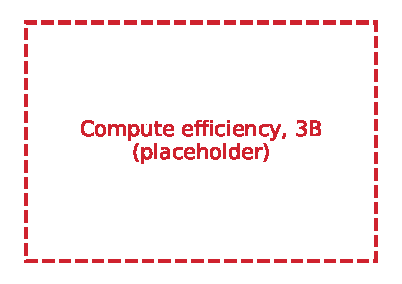
\includegraphics[width=0.33\linewidth]{figures/vt_efficiency_3b.pdf}
		\label{fig:vt_efficiency_3b}
	}
	\hspace{-0.25in}
	\hfill
	\subfigure[Qwen2.5-VL-7B on Jetson AGX Orin]{
		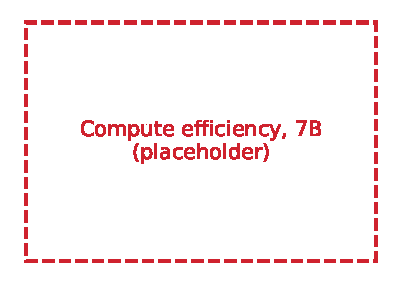
\includegraphics[width=0.33\linewidth]{figures/vt_efficiency_7b.pdf}
		\label{fig:vt_efficiency_7b}
	}
	\hspace{-0.25in}
	\hfill
	\subfigure[Qwen2.5-VL-32B-4bit on Jetson AGX Orin]{
		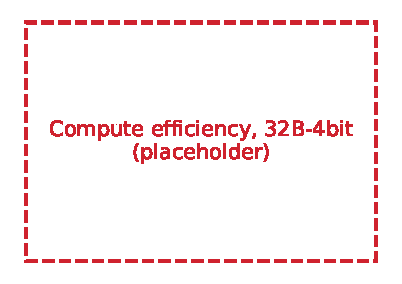
\includegraphics[width=0.33\linewidth]{figures/vt_efficiency_32b.pdf}
		\label{fig:vt_efficiency_32b}
	}
	\hspace{-0.25in}
	\vspace{-0.15in}
	\caption{Compute efficiency on Jetson AGX Orin with different VLM backbones}
	\vspace{-0.1in}
	\label{fig:vt_efficiency}
\end{figure*}

\vspace{-0.1in}
\subsection{On-Device Compute Efficiency}
\label{sec:efficiency}

Figure~\ref{fig:vt_efficiency} presents the compute latency, energy, and memory cost of ViewTree and the baselines on Jetson AGX Orin...

\begin{figure*}[ht]
	\vspace{-0.1in}
	\centering
	\subfigure[Object Number]{
		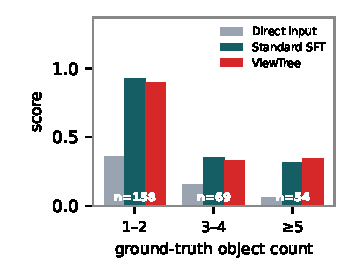
\includegraphics[width=0.30\linewidth]{figures/vt_object_number.pdf}
	}
	\hspace{-0.25in}
	\hfill
	\subfigure[Spatial Scale]{
		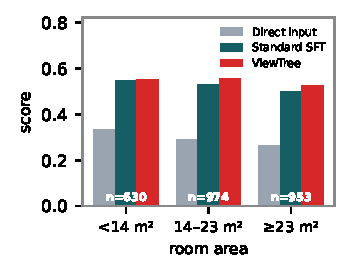
\includegraphics[width=0.30\linewidth]{figures/vt_spatial_scale.pdf}
	}
	\hspace{-0.25in}
	\hfill
	\subfigure[Temporal Duration]{
		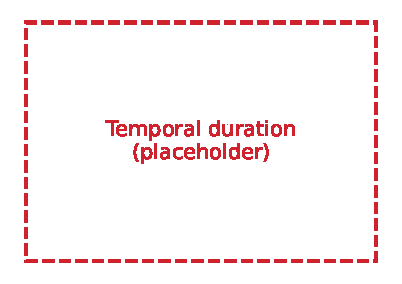
\includegraphics[width=0.30\linewidth]{figures/vt_temporal_duration.pdf}
	}
	\vspace{-0.15in}
	\caption{Spatial task performance with different levels of scene complexities}
	\vspace{-0.1in}
	\label{fig:vt_complexity}
\end{figure*}

\subsection{Performance over Different Levels of Scene Complexities}
\label{sec:complexity}

We analyze how the scene complexity affects the spatial task performance, using the Qwen2.5-VL-7B backbone on the VSI-Bench....

\vspace{-0.1in}
\subsection{Ablation Studies}
\label{sec:ablation}

\noindent\textbf{Different view-acquisition strategies.} To validate the effectiveness of confidence-guided beam search over camera walks, we compare it against (1) presenting all five candidate views unconditionally (static memory), (2) a random walk of the same depth budget, and (3) greedy walk (beam width 1), on the VSI-Bench held-out split. As shown in Table~\ref{tab:vt_keyview_ablation}, ...

\begin{table}[h]
	\vspace{0.1in}
	\centering
	\small
	\begin{minipage}[t]{0.48\textwidth}
		\centering
		\begin{tabular}{lcc}
			\toprule
			\textbf{Qwen2.5-VL-7B} & \textbf{Task accuracy} & \textbf{VLM calls} \\ \midrule
			All views (static)          & --            & --              \\
			Random walk                 & --            & --              \\
			Greedy walk (b=1)           & --            & --              \\
			\textbf{Ours }   & \textbf{--}   & --              \\ \bottomrule
		\end{tabular}
		\label{tab:vt_ablation_view_7B}
	\end{minipage}
	\hfill
	\begin{minipage}[t]{0.48\textwidth}
		\centering
		\begin{tabular}{lcc}
			\toprule
			\textbf{Qwen2.5-VL-32B-4bit} & \textbf{Task accuracy} & \textbf{VLM calls} \\ \midrule
			All views (static)          & --            & --              \\
			Random walk                 & --            & --              \\
			Greedy walk (b=1)           & --            & --              \\
			\textbf{Ours}   & \textbf{--}   & --              \\ \bottomrule
		\end{tabular}
		\label{tab:vt_ablation_view_32B}
	\end{minipage}
	\vspace{0.05in}
	\caption{Ablation of view-acquisition strategies on the VSI-Bench held-out split.}
	\label{tab:vt_keyview_ablation}
	\vspace{-0.15in}
\end{table}

\noindent\textbf{Component ablations.} Table~\ref{tab:vt_component_ablation} isolates the contribution of each ViewTree component on the VSI-Bench ...

\begin{table}[h]
	\centering
	\small
	\begin{tabular}{lcc}
		\toprule
		\textbf{Variant} & \textbf{Avg accuracy} & \textbf{VLM calls} \\ \midrule
		\textbf{ViewTree-D (full)}          & \textbf{--} & -- \\
		\;\;w/o exploration gate            & --          & -- \\
		\;\;w/o confidence head (token prob.)& --         & -- \\
		\;\;w/o human-camera constraint     & --          & -- \\
		\;\;depth capped at 1               & --          & -- \\
		\;\;w/o direct-answer arbitration   & --          & -- \\ \bottomrule
	\end{tabular}
	\caption{Component ablations on the VSI-Bench held-out split (Qwen2.5-VL-7B).}
	\label{tab:vt_component_ablation}
	\vspace{-0.2in}
\end{table}
	
	
	
	
	\bibliographystyle{ACM-Reference-Format}
	\bibliography{main,mobicom26}
	
\end{document}
